% Author: Izaak Neutelings (October 2020)
% Inspiration: https://courses.lumenlearning.com/physics/chapter/9-3-stability/
\documentclass[border=3pt,tikz]{standalone}
\usepackage{physics}
\usepackage{siunitx}
\usepackage{tikz}
\usepackage[outline]{contour} % glow around text
\usetikzlibrary{calc}
\usetikzlibrary{angles,quotes} % for pic
\usetikzlibrary{arrows.meta}
\usetikzlibrary{patterns}
\tikzset{>=latex} % for LaTeX arrow head
\contourlength{1.35pt}

\colorlet{xcol}{blue!70!black}
\colorlet{vcol}{green!60!black}
\colorlet{myred}{red!65!black}
\colorlet{mydarkred}{red!45!black}
\colorlet{mypurple}{blue!60!red!80}
\colorlet{acol}{red!50!blue!80!black!80}
\tikzstyle{rvec}=[->,xcol,very thick,line cap=round]
\tikzstyle{vvec}=[->,vcol,very thick,line cap=round]
\tikzstyle{myarr}=[{Latex[length=3,width=3]}-,xcol]
\tikzstyle{myarr2}=[{Latex[length=2,width=3]}-{Latex[length=2,width=3]}]
\tikzstyle{force}=[->,myred,very thick,line cap=round]
\tikzstyle{Fproj}=[force,myred!40]
\tikzstyle{myarr}=[{Latex[length=3,width=3]}-]
\tikzstyle{CM}=[red!40!black,fill=red!80!black!80]
\tikzstyle{mydashed}=[dash pattern=on 2 off 2]
\tikzstyle{mass}=[line width=0.6,draw=red!30!black,rounded corners=1,
                  top color=red!40!black!30,bottom color=red!40!black!10,shading angle=30]
\tikzstyle{ground}=[preaction={fill,top color=black!10,bottom color=black!5,shading angle=20},
                    fill,pattern=north east lines,draw=none,minimum width=0.3,minimum height=0.6]
\tikzstyle{metal}=[fill,top color=black!40,bottom color=black!20,shading angle=10]
\def\tick#1#2{\draw[thick] (#1) ++ (#2:0.1) --++ (#2-180:0.2)}


\def\r{0.05} % pulley small radius
\tikzset{
  pics/Tin/.style={
    code={
      \def\R{0.12}
      \draw[pic actions,line width=0.6,#1,fill=white] % ,thick
        (0,0) circle (\R) (-135:.75*\R) -- (45:.75*\R) (-45:.75*\R) -- (135:.75*\R);
  }},
  pics/Tout/.style={
    code={
      \def\R{0.12}
      \draw[pic actions,line width=0.6,#1,fill=white] (0,0) circle (\R);
      \fill[pic actions,#1] (0,0) circle (0.3*\R);
  }},
  pics/rotarr/.style={
    code={
      \draw[white,very thick] ({#1*cos(200)},0) arc(-200:30:{#1} and {#1/2}) --++ (125:0.1);
      \draw[->] ({#1*cos(200)},0) coordinate (W1) arc(-200:20:{#1} and {#1/2}) node[midway] (W2) {} --++ (125:0.1) coordinate (W3);
  }},
  pics/Tin/.default=mypurple,
  pics/Tout/.default=mypurple,
  pics/rotarr/.default=0.4,
}

\begin{document}


% BLOCK - metastable
\def\H{3.1} % block height
\def\W{1.4} % block width
\def\R{sqrt(\W^2+\H^2)/2} % block half-diagonal
\def\D{0.25} % ground depth
\def\ang{atan(\H/\W)} % angle diagonal ccw
\def\angcw{atan2(\H,-\W)} % angle diagonal cw
\begin{tikzpicture}
  \coordinate (O) at (0,0);
  \coordinate (CM) at (0,\H/2);
  \coordinate (BL) at (-\W/2,0); % bottom left corner
  \coordinate (BR) at (\W/2,0); % bottom right corner
  \coordinate (TR) at (\W/2,0); % top right corner
  \draw[ground] (-0.8*\W,0) rectangle (1.4*\W,-\D);
  \draw[thick] (-0.8*\W,0) -- (1.4*\W,0);
  \draw[mass] (-\W/2,0) rectangle++ (\W,\H);
  \node[left] at (-\W/2,\H/2) {$W$};
  \node[above] at (0,\H) {$H$};
  \draw[CM] (CM) circle(0.06*\W);
  \draw[dashed] (BR) -- (CM) --++ ({\angcw}:0.2*\W);
  \draw[dashed] (BR)++(130:{\R}) arc(130:35:{\R});
  \draw pic[myarr,"$\theta$"scale=0.9,draw,angle radius=18,angle eccentricity=1.35] {angle=TR--BR--CM};
  \draw[force] (CM) --++ (0,-0.24*\H) node[midway,below=2,left=-1] {$m\vb{g}$};
  \draw[force] (O) --++ (0,0.24*\H) node[midway,left=-1] {$\vb{F}_\mathrm{N}$};
  \node[mypurple,above right=2] at (BR) {$\vb*\tau=0$};
  %\draw[->] (F)++(42:1.9*\L) arc(70:0:0.5*\L) node[midway,above right=-2] {$\alpha$};
  \draw[rvec] (BR) -- (CM) node[below=6,right=4] {$\vb{r}$};
  \draw[rvec] (BR) -- (O) node[midway,above=-2.2] {$\vb{r}_\mathrm{t}$};
  %\draw[rvec] (BR) -- (O) node[midway,right=2,below=-1.5] {\contour{white}{$\vb{r}_\mathrm{t}$}};
  \fill[blue!50!black] (BR) circle(0.03*\W);
\end{tikzpicture}


% BLOCK - torque
\begin{tikzpicture}
  \def\ang{11}
  \coordinate (CM) at ({\angcw-\ang}:{\R});
  \coordinate (BR) at (0,0); % bottom right corner
  \coordinate (BL) at ({180-\ang}:\W); % bottom left corner
  \coordinate (TR) at ({\ang}:\W); % bottom left corner
  \coordinate (T) at ({\angcw-\ang-8}:{1.15*\R}); % torque 
  \draw[ground] (-1.3*\W,0) coordinate (L) rectangle (0.9*\W,-\D);
  \draw[thick] (-1.3*\W,0) -- (0.9*\W,0);
  \draw[mass,rotate around=({-\ang}:(BR))]
    (-\W,0) rectangle++ (\W,\H);
  \draw[CM] (CM) circle(0.06*\W);
  \draw[dashed] (BR) --++ (0,{1.6*\R});
  \draw[dashed] (BR)++(120:{\R}) arc(120:40:{\R});
  \draw[force] (CM) --++ (0,-0.24*\H) node[midway,below=2,left=-1] {$m\vb{g}$};
  \draw[force] (BR) --++ (0,0.24*\H) node[below right=0] {$\vb{F}_\mathrm{N}$};
  \pic[scale=1] at (T) {Tin};
  \node[mypurple,above=1] at (T) {$\vb*\tau$};
  \draw pic[myarr,draw,angle radius=35,angle eccentricity=1.1] {angle=BL--BR--L};
  \draw[rvec] (BR) -- (CM) node[midway,below left=-2] {$\vb{r}$};
  \draw[->] (110:1.1*\H) arc(110:148:0.4*\H) node[above left=-1] {$\alpha$};
  \fill[blue!50!black] (BR) circle(0.03*\W);
\end{tikzpicture}


% BLOCK - unstable
\begin{tikzpicture}
  \coordinate (CM) at (0,{\R});
  \coordinate (BR) at (0,0); % bottom right corner
  \coordinate (BL) at ({90+\ang}:\W); % bottom left corner
  \coordinate (TR) at ({\ang}:\W); % bottom left corner
  \coordinate (T) at (0.2*\W,{1.2*\R}); %(30:0.3*\W); % torque
  \coordinate (R) at (\W,0); % bottom left corner
  \draw[ground] (-1.1*\W,0) coordinate (L) rectangle (1.2*\W,-\D);
  \draw[thick] (-1.1*\W,0) -- (1.2*\W,0);
  \draw[mass,rotate around=({90-\angcw}:(BR))]
    (-\W,0) rectangle++ (\W,\H);
  \draw[CM] (CM) circle(0.06*\W);
  \draw[dashed] (BR) --++ (0,{1.2*\R});
  \draw[dashed] (BR)++(120:{\R}) arc(120:40:{\R});
  \draw[force] (CM) --++ (0,-0.24*\H) node[midway,below=2,left=-1] {$m\vb{g}$};
  \draw[force] (BR) --++ (0,0.24*\H) node[left=-2] {$\vb{F}_\mathrm{N}$};
  \node[mypurple,above=-1] at (T) {$\vb*\tau=0$};
  \draw pic[<-,draw,angle radius=20,angle eccentricity=1.3] {angle=BL--BR--L};
  \fill[blue!50!black] (BR) circle(0.03*\W);
  \draw pic["$\phi$",draw,angle radius=11,angle eccentricity=1.45] {angle=R--BR--TR};
\end{tikzpicture}


% BLOCK - stable
\begin{tikzpicture}
  \coordinate (O) at (0,0);
  \coordinate (CM) at (0,\W/2);
  \coordinate (BL) at (-\H/2,0); % bottom left corner
  \coordinate (BR) at (\H/2,0); % bottom right corner
  \draw[ground] (-0.8*\H,0) rectangle (0.8*\H,-\D);
  \draw[thick] (-0.8*\H,0) -- (0.8*\H,0);
  \draw[mass] (-\H/2,0) rectangle++ (\H,\W); %,shading angle=80
  \draw[CM] (CM) circle(0.06*\W);
  \draw[dashed] (BL) -- (CM) --++ ({atan(\W/\H)}:0.14*\W);
  \draw[dashed] (BL)++(120:{\R}) arc(120:25:{\R});
  \draw[force] (CM) --++ (0,-0.24*\H)
    node[midway,below=3,left=0] {\contour{red!40!black!19}{$m\vb{g}$}};
  \draw[force] (O)++(0.14*\W,0) --++ (0,0.24*\H) node[midway,right=-1] {$\vb{F}_\mathrm{N}$};
  \node[mypurple,above=1,above right=0] at (CM) {$\vb*\tau=0$};
  \fill[blue!50!black] (BL) circle(0.03*\W);
\end{tikzpicture}


% BLOCK - plot
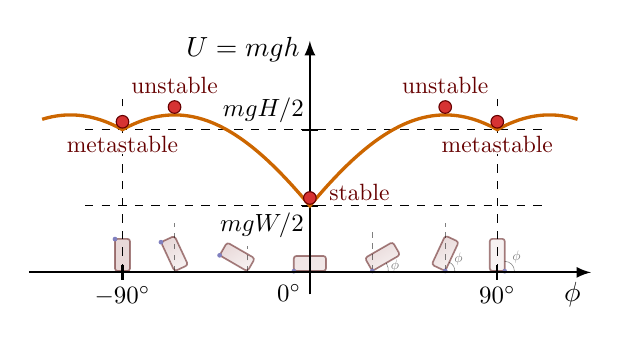
\begin{tikzpicture}
  \def\xmax{3.4}
  \def\ymax{2.8}
  \def\angms{25}            % unstable angle
  \def\angus{atan(tan(\angms))} % unstable angle
  \def\angne{60}            % non-equilibrium
  \def\A{2.0}               % amplitude / yscale
  \def\yW{\A*sin(\angms)}   % y position phi =  0
  \def\yH{\A*cos(\angms)}   % y position phi = 90
  \def\xH{0.7*\xmax}        % x position phi = 90
  \def\xi{(90-\angms)/\om}  % x position unstable
  \def\om{(90/(\xH))}
  \def\h{0.12*\xmax} % height mini block
  \def\w{\h*tan(\angus)} % width mini block
  \coordinate (O) at (0,0);
  \coordinate (P-2) at ({(\angus-90)/\om},0.014);
  \coordinate (P-1) at ({(\angne-90)/\om},0.013);
  \coordinate (P+1) at ({(90-\angne)/\om},0.018);
  \coordinate (P+2) at ({(90-\angus)/\om},0.018);
  
  % MASS BLOCKS
  \begin{scope}[opacity=0.5]
    \draw[mass,rounded corners=0.9]
      ({-\xH-\w/2},0.018) rectangle++ ({\w},\h) % phi = -90
      (-\h/2,0.018) rectangle++ (\h,{\w})       % phi = 0
      ({\xH-\w/2},0.018) rectangle++ ({\w},\h); % phi = +90
    \draw[mass,rotate around={{\angus}:(P-2)}]
      (P-2) rectangle++ ({\w},\h);
    \draw[mass,rotate around={{\angne}:(P-1)}]
      (P-1) rectangle++ ({\w},\h);
    \draw[mass,rotate around={{-\angne}:(P+1)}]
      (P+1) rectangle++ (-{\w},\h);
    \draw[mass,rotate around={{-\angus}:(P+2)}]
      (P+2) rectangle++ (-{\w},\h);
    \draw[very thin]
      ({\xH+\w/2+0.3*\h},0.018) arc(0:90:0.3*\h) node[pos=0.5,above right=-1.4,scale=0.5] {$\phi$}
      (P+1)++(-5:0.50*\h) arc(-5:{90-\angne}:0.50*\h) node[pos=0.7,right=-0.5,scale=0.5] {$\phi$}
      (P+2)++(-5:0.30*\h) arc(-5:{90-\angus}:0.30*\h) node[pos=0.5,above right=-1.4,scale=0.5] {$\phi$};
    \draw[very thin,mydashed]
      (P-2) --++ (0,1.5*\h)
      (P-1) --++ (0,0.8*\h)
      (P+1) --++ (0,1.2*\h)
      (P+2) --++ (0,1.5*\h);
  \end{scope}
  \fill[blue!50!black!50]
    ({-\xH-\w/2},\h+0.015) circle (0.03)
    (-\h/2,0.015) circle (0.03)
    (P-2)++({90+\angus}:\h) circle (0.03)
    (P-1)++({90+\angne}:\h) circle (0.03)
    (P+1) circle (0.03)
    (P+2) circle (0.03)
    ({\xH+\w/2},0.015) circle (0.03);
  
  % PLOT
  \draw[->,thick] (0,-0.1*\ymax) -- (0,1.05*\ymax) node[below=3,left] {$U=mgh$};
  \draw[->,thick] (-1.05*\xmax,0) -- (1.05*\xmax,0) node[below left] {$\phi$}; %$[\si{\degree}]$ %\theta
  \tick{-\xH,0}{90} node[below=-1,scale=0.9] {$\SI{-90}{\degree}$};
  \tick{\xH,0}{90} node[below=-1,scale=0.9] {$\SI{90}{\degree}$};
  \node[below=1,below left,scale=0.9] at (O) {$\SI{0}{\degree}$};
  \draw[dashed] (-\xH,0) --++ (0,1.1*\A);
  \draw[dashed] (\xH,0) --++ (0,1.1*\A);
  \tick{0,{\yH}}{0} node[right=3,above left=-1,scale=0.9] {$mgH/2$};
  \tick{0,{\yW}}{0} node[right=3,below left=-1,scale=0.9] {$mgW/2$};
  \draw[dashed] (-1.2*\xH,{\yH}) -- (1.24*\xH,{\yH});
  \draw[dashed] (-1.2*\xH,{\yW}) -- (1.24*\xH,{\yW});
  \draw[very thick,orange!80!black,samples=100,smooth,variable=\t]
    plot[domain=-\xmax:-\xH](\t,{\A*sin(\om*abs(\t)-\angms)}) --
    plot[domain=-\xH:0](\t,{\A*sin(\om*abs(\t)+\angms)}) --
    plot[domain=0:\xH](\t,{\A*sin(\om*\t+\angms)}) --
    plot[domain=\xH:\xmax](\t,{\A*sin(\om*\t-\angms)}); %node[right] {$x$}
    
  % CENTER OF MASS
  \draw[CM] (-\xH,{\yH+0.1}) circle(0.08) node[below=4,scale=0.85,fill=white,inner sep=1] {metastable};
  \draw[CM] (\xH,{\yH+0.1}) circle(0.08) node[below=4,scale=0.85,fill=white,inner sep=1] {metastable};
  \draw[CM] ({(90-\angms)/\om},{\A+0.1}) circle(0.08) node[above=2,scale=0.85] {unstable};
  \draw[CM] ({(\angms-90)/\om},{\A+0.1}) circle(0.08) node[above=2,scale=0.85] {unstable};
  \draw[CM] (0,{\yW+0.1}) circle(0.08) node[above=2,right=4,scale=0.85] {stable};
  
\end{tikzpicture}


\end{document}
